\documentclass[12pt]{beamer}

\usepackage{algpseudocode}
\usepackage{algorithm2e}

\author{Jake Humphrey}
\title{A Stochastic Computational Approach for Accurate and Efficient Reliability Evaluation}
\subtitle{A Python Implementation}
\institute{Department of Electronic and Electrical Engineering\\
  Imperial College London\\
  \texttt{jbh111@ic.ac.uk}
}

\begin{document}

\begin{frame}[plain]
  \titlepage
\end{frame}

\begin{frame}{Reliability of Circuits}
Gates in a logic circuit are susceptible to errors:
\begin{itemize}
\item \textbf{Stuck-At-One Error:} Output goes high.
\item \textbf{Stuck-At-Zero Error:} Output goes low.
\item \textbf{Von Neumann Error:} Output is inverted.
\end{itemize}
\end{frame}

\begin{frame}{Masking Effects}
However, the error may not affect the output due to one of the following \emph{masking effect}s
\begin{itemize}
\item \textbf{Electrical Masking:} Error signal too weak to be detected.
\item \textbf{Temporal Masking:} Error misses the detection window of a latch.
\item \textbf{Logical Masking:} The error does not change the output of a logic gate.
\end{itemize}
\end{frame}
\begin{frame}{Reliability Analysis \small Principles}
Logical Masking is the most common, and so we try to analyse circuits on their ability to logically mask errors.
\vspace{0.25cm}

\emph{Probability} of a signal = chance that it is logically True.

\emph{Reliability} of a signal = chance that it takes the correct value
\vspace{0.25cm}

\begin{itemize}
\item Construct an error-prone representation of the circuit.
\item Derive the \emph{probabilities} of the outputs from the inputs.
\item Find the output \emph{reliabilities}.
\end{itemize}
\end{frame}

\begin{frame}{Reliability Analysis \small Probabilistic Gate Models}
\only<1>{
However, existing algorithms are inefficient!
\vspace{0.25cm}

For example, \emph{Probabilistic Gate Models} (PGMs) attempt to derive the output probabilities deterministically and analytically.
}
\only<2>{
The problem occurs when the inputs to a gate are statistically dependent.
\vspace{0.25cm}

The PGM equations do not account for statistically dependent signals, and the solution involves splitting the circuit into two sub-circuits, doubling the cost of the algorithm.
}
\end{frame}

\begin{frame}{Reliability Analysis \small Stochastic Computing}
The use of \emph{Stochastic Computing} can avoid these issues. 
\vspace{0.25cm}

Generate input bitstreams and propagate them through the circuit.
\vspace{0.25cm}

The output probabilities can then be accurately calculated from the output bitstreams.
\end{frame}

\begin{frame}{Reliability Analysis \small Stochastic Logic with Bernoulli Sequences}

Existing Stochastic Logic algorithms use the input probabilities to generate \emph{Bernoulli Sequences} of the form:

\begin{equation*}
[X_0, X_1 \dots X_{n-1}]; X_i \sim B(p)
\end{equation*}

for each input, where $p$ is the input probability.
\vspace{0.25cm}

Requires $n$ random numbers must be generated for each input!
\end{frame}

\begin{frame}{Reliability Analysis \small Stochastic Logic with Non-Bernoulli Sequences}
\emph{Non-Bernoulli Sequences} reduce the random number generation overhead.
\vspace{0.25cm}

They are generated deterministically with the expected number of 1s, and then randomly permuted.
\vspace{0.25cm}

Only one random number generation is required per input bitstream!
\end{frame}

\begin{frame}{Reliability Analysis Algorithm}
Using Stochastic Computation with Non-Bernoulli Sequences, we arrive at an algorithm for Reliability Analysis, which I will describe over the following slides.
\end{frame}

\begin{frame}[fragile]{Reliability Analysis Algorithm \small Pseudocode}
\begin{algorithm}[H]
\KwData{Logic circuit to be tested}
\KwResult{Reliabilities for each output}
\For{each gate in the circuit}{represent gate in faulty circuit\;}
\For{each input to the faulty circuit}{generate a non-Bernoulli sequence\;}
\For{each output in the circuit}{
	\For{each input vector}{
		\If{outputs are the same for each circuit}{add 1/n to reliability of that output\;}
	}
}
\end{algorithm}
\end{frame}

\begin{frame}{Reliability Analysis Algorithm \small Complexity Analysis}
The most costly section is the final double loop!
\vspace{0.25cm}

We have to propagate a signal through each circuit once for each output, and $n$ times.
\vspace{0.25cm}

Could be at worst $O(ogn)$, where:

$o$ = number of outputs

$n$ = length of Non-Bernoulli Sequences

$g$ = number of gates
\end{frame}

\begin{frame}[fragile]{Reliability Analysis Algorithm \small Further Work}
Still has room for improvement: inputs propagates through circuit once per output
\vspace{0.25cm}

It has to redundantly recalculate many intermediate values!
\vspace{0.25cm}

Calculating all the output values in one go would reduce the double loop to a single one over the length of the input sequences.
\vspace{0.25cm}

This reduces the algorithm complexity to $O(gn)$
\end{frame}

\begin{frame}{Reliability Analysis Algorithm \small Runtime Analysis}
\center
\only<1>{
\begin{tabular}{l|r r}
	Input Files & c17.v& c432.v\\
  \hline
  Inputs & 5 & 36\\
  Outputs & 2 & 7\\
  Gates & 6 & 160\\
  \hline
  Input Sequence Length & runtime /s & runtime /s\\
  \hline
  1 & 0.00023 & 1.34\\
  10 & 0.00067 & 12.2\\
  100 & 0.00485 & 122\\
  1 000 & 0.0473 & 1250\\
  10 000 & 0.458 & No Data\\
  100 000 & 4.66 & No Data
\end{tabular}}
\only<2>{
\begin{figure}
  \centering
    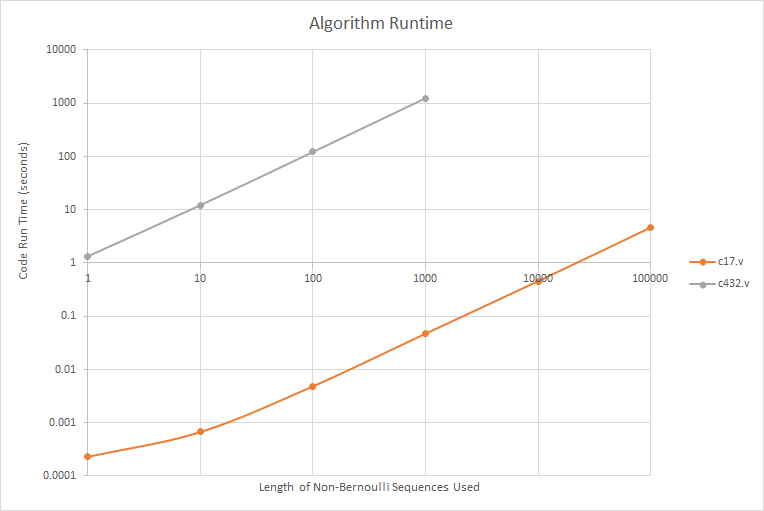
\includegraphics[width=\textwidth]{runtime}
\end{figure}
}
\end{frame}
\end{document}